\documentclass{beamer}
\usetheme{Szeged}
\usecolortheme{beaver}

\usepackage{graphicx}
\usepackage[center]{caption}

\title{k-anonymity in go}
\titlegraphic{
  
\includegraphics{../images/gopher-anon.png}
}

\date{April, 2019}
\author{Richard Garai}
\institute[BME / AUT]{
  Budapest University of Technology and Economics\\
  Department of Automation and Applied Informatics
  }


\begin{document}

\frame{\titlepage}

\section{k-anonymity}

\begin{frame}
  \frametitle{privacy is ever more important}
  \begin{columns}
    \column{.6\textwidth}
    \begin{itemize}
      \item{tremendous growth in collection and analysis of personal data\cite{aggarwal}}
        \begin{itemize}
          \item[-]{cloud services}
          \item[-]{mobile apps}
	  \item[-]{smart fridge}
	  \item[-]{etc\ldots}
        \end{itemize}
      \item{new regulations}
	\begin{itemize}
	  \item[-]{EU: GDPR\cite{wiki-anon}}
        \end{itemize}
    \end{itemize}
    \column{.4\textwidth}
    \begin{figure}
      
\includegraphics{../images/gopher-multimedia.png}
    \end{figure}
  \end{columns}
\end{frame}

\begin{frame}
  \frametitle{data anonymization}  
  \begin{columns} 
    \column{.6\textwidth}
    \begin{block}{medical data}
      \vspace{10pt} 
      \tiny
      \begin{tabular}{ c|c|c|c|c|c }
        \textbf{name} & \textbf{age} & \textbf{race} & \textbf{gender} & \textbf{zip} & \textbf{disease} \\
        \hline
	\color{orange} John & 47 & white & male & 1077 & \color{violet} cancer \\
        \hline
	\color{orange} Sandy & 35 & white & female & 1077 & \color{violet} flu \\
        \hline
	\color{orange} Mary & 27 & asian & female & 1095 & \color{violet} flu \\
        \hline
	\color{orange} Janet & 27 & white & female & 1095 & \color{violet} hypertension 
      \end{tabular}
    \end{block}   
    \column{.4\textwidth}
    \begin{itemize}
      \item{\color{orange} identifier}
      \item quasi-identifier
      \item{\color{violet} non-identifier}
    \end{itemize}
  \end{columns} 
  \vspace{20pt}
  \begin{columns}
    \column{.6\textwidth}
    \begin{block}{anonymized medical data}
      \vspace{10pt}
      \tiny
        \begin{tabular}{ c|c|c|c|c|c }
        \textbf{name} & \textbf{age} & \textbf{race} & \textbf{gender} & \textbf{zip} & \textbf{disease} \\
        \hline
	\color{red} * & \color{blue} 30..50 & white & \color{red} * & 1077 & cancer \\
        \hline
        \color{red} * & \color{blue} 30..50 & white & \color{red} * & 1077 & flu \\
        \hline
        \color{red} * & 27 & \color{red} * & female & 1095 & flu \\
        \hline
        \color{red} * & 27 & \color{red} * & female & 1095 & hypertension 	
      \end{tabular} 
    \end{block}
    \column{.4\textwidth}
    \begin{itemize}
      \item{\color{red} suppression}
      \item{\color{blue} generalization}
    \end{itemize}
  \end{columns}    
\end{frame}

\begin{frame}
  \frametitle{definition of k-anonimity}
  \begin{block}{k-anonimity}
    \textit{suppress/generalize entries in the table until for each row, there are at least \textcolor{red}{k-1} other rows that are identical to it along the quasi-identifying attributes}
  \end{block}
  \begin{columns}
    \column{.6\textwidth}
    \begin{block}{}
      \begin{itemize}
        \item{k-anonymity even with only suppression and a ternary alphabet, i.e. \(\Sigma = \{0, 1, 2\}\) is NP-hard \cite{aggarwal} }
      \end{itemize}
    \end{block}
    \column{.4\textwidth}
    \begin{figure}
      
\includegraphics[width=100px]{../images/gopher-calc.png}
    \end{figure}
  \end{columns}
\end{frame}


\section{algorithm}

\begin{frame}
  \frametitle{cost graph}
  \begin{columns}
    \column{.5\textwidth}
    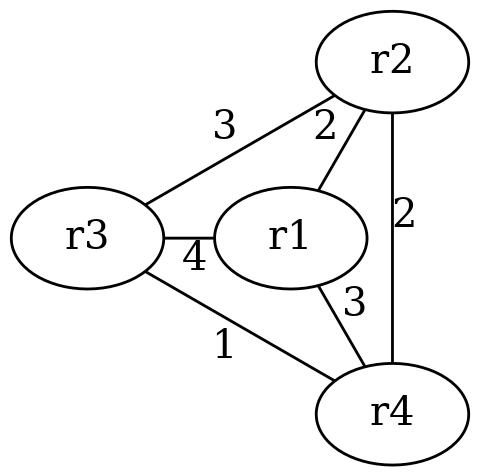
\includegraphics[width=140px]{../graphs/cost-graph.png}
    \column{.5\textwidth}
    \begin{block}{edge weight}
      $$w(e)=\sum_{j}^{} \frac{h_{a,b}(j)}{l_{j}}$$ \\
      \scriptsize{
	\textcolor{red}{ \(h_{a,b}\) } generalization cost of items a and b \\
	\textcolor{red}{ \(l_{j}\) } maximum levels of generalization for column j
      }
    \end{block}
  \end{columns}
\end{frame}

\begin{frame}
  \frametitle{forest building}
  \begin{center}
    \begin{figure}[ht]
      \begin{overlayarea}{150px}{150px}
	\includegraphics<1>[width=140px]{../graphs/cost-graph-s0.png}
	\includegraphics<2>[width=140px]{../graphs/cost-graph-s1.png}
	\includegraphics<3>[width=140px]{../graphs/cost-graph-s2.png}
	\includegraphics<4>[width=140px]{../graphs/cost-graph-s3.png}
	\includegraphics<5>[width=140px]{../graphs/cost-graph-s4.png}  
	\includegraphics<6>[width=140px]{../graphs/cost-graph-s5.png}
      \end{overlayarea}
    \end{figure}
  \end{center}
\end{frame}

\begin{frame}
  \frametitle{partition refinement}
  \begin{columns}
  \column{.6\textwidth}
  	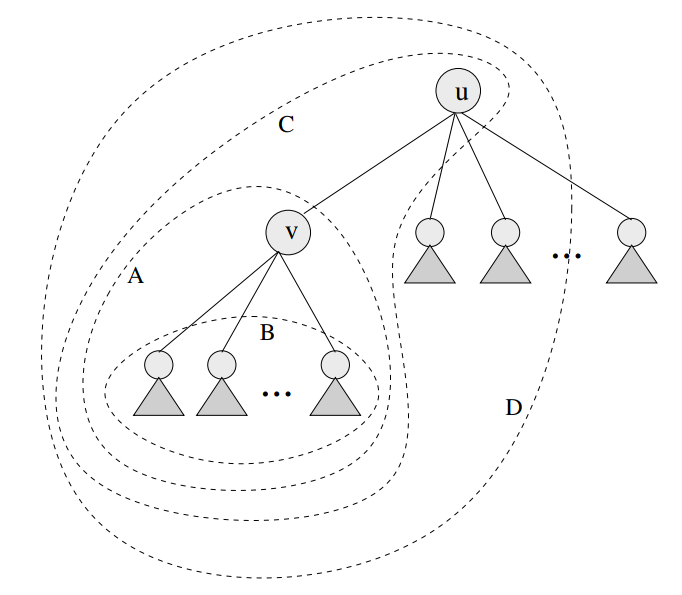
\includegraphics[width=180px]{../images/graph-cuts.png}
  \column{.4\textwidth}
  large components are refined further
  $$ s > max\{2k-1,3k-5\} $$
  \begin{itemize}
    \item 4 distinct cut types
    \item  Steiner's Vertices \cite{aggarwal}
  \end{itemize}
  \end{columns}
\end{frame}

\section{api}

\begin{frame}[fragile]
  \frametitle{anonymization example code}
  \begin{columns}
  \column{.65\textwidth}
  \scriptsize
  \begin{verbatim}
table := model.NewTable(&model.Schema{
   Columns: []*model.Column{
      model.NewColumn("col", &generalizer),
      [...]
   },
	})
	
table.AddRow(item1, item2, ...)


anon := &Anonymizer{
   Table: table,
   K:     2,
}
	err := anon.Anonymize()
  \end{verbatim}
  \column{.35\textwidth}
  generalizers:
  \begin{itemize}
    \item suppressor
    \item int range
    \item float range
    \item string prefix
    \item \textcolor{red}{hierarchy}
  \end{itemize}
  \end{columns}
\end{frame}

\section{integration}
\begin{frame}
  \frametitle{integration with existing anonymization system}
  \begin{figure}[h!]
  \begin{center}
  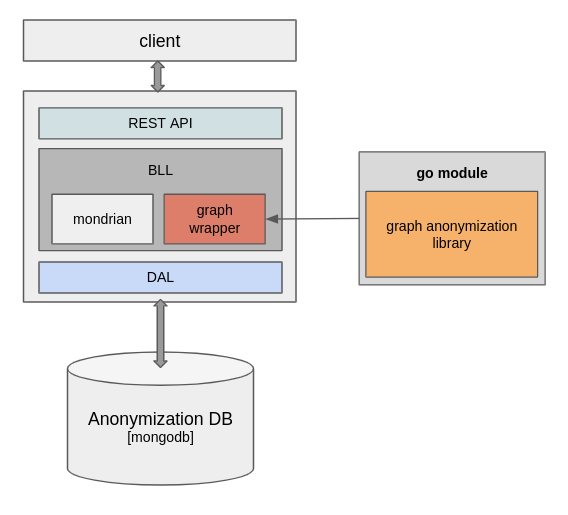
\includegraphics[height=200px]{../images/components.png}
  \end{center}
  \end{figure}
\end{frame}

\section{closing notes}
\begin{frame}
  \frametitle{future improvements, references}
  \begin{columns}  
  \column{.6\textwidth}
  \begin{itemize}
    \item optimized algorithm for special cases
    \begin{itemize}
      \item[-]k = 2
      \item[-]k = 3
    \end{itemize}
    \item continous anonymization (\checkmark done)
    \item anonymization of streaming data
  \end{itemize}
  \column{.4\textwidth}
  
\includegraphics[width=120px]{../images/gophers.png}
  \end{columns}
  \vspace{10pt}
  \begin{thebibliography}{2}
  \bibitem{aggarwal}
  \scriptsize
  \textit{Approximation Algorithms for k-Anonymity}\\
  Gagan Aggarwal, Tomas Feder, Krishnaram Kenthapadi, Rajeev Motwani, Rina Panigrahy, Dilys Thomas, An Zhu
  Journal of Privacy Technology, 2015.

  \bibitem{wiki-anon}
    \textit{Data Anonymization}\\
    Wikipedia Article (https://en.wikipedia.org/wiki/Data\_anonymization)

  \end{thebibliography}

\end{frame}

\end{document}
